\documentclass[tikz,border=10pt]{standalone}
\usetikzlibrary{calc}
\begin{document}
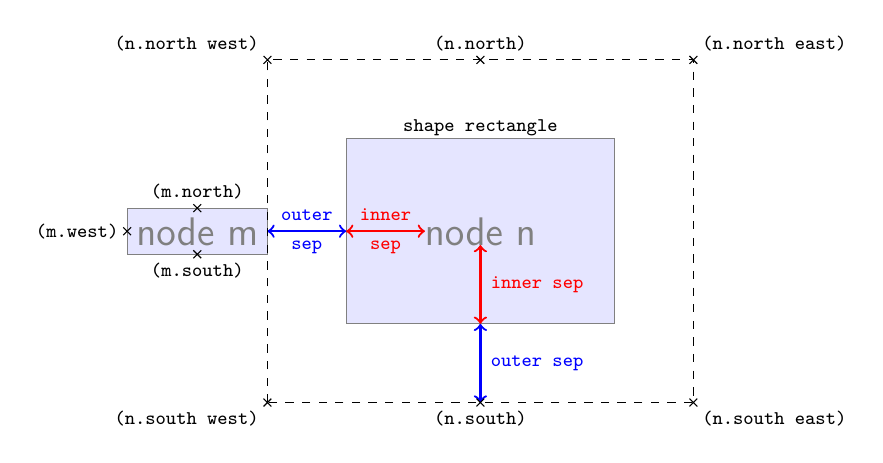
\begin{tikzpicture}[font={\scriptsize\ttfamily}]
\node[draw,rectangle,outer sep=1cm,inner sep=1cm,color=black!50, draw, fill=blue!10,]
  (n) {{\sffamily\Large node n}};

\draw[<->,thick,blue] (n.south)
    --++(0,1cm) node[midway,right]{outer sep};

\draw[<->,thick,red] (n.south) ++(0,1cm) 
    --++(0,1cm)node[midway,right]{inner sep};
    
\node[,outer sep=0,draw,left,color=black!50, draw, fill=blue!10,] 
    (m) at(n.west) {{\sffamily\Large node m}};
    
\draw[<->,blue,thick] (m.east) -- ++(1cm,0) node[midway,above] {outer}
  node[midway,below] {sep};

\draw[<->,red,thick] ($(n.west)+(1,0)$) -- ++(1cm,0) node[midway,above] {inner}
  node[midway,below] {sep};

\foreach \anchor/\placement in
  {south west/below left,south/below,north/above,north west/above left,
     north east/above right,south east/below right}
     \draw[shift=(n.\anchor)] plot[mark=x] coordinates{(0,0)}
      node[\placement,label distance = 0mm,inner sep=3pt] {(n.\anchor)};
\foreach \anchor/\placement in
  {west/left,south/below,north/above}
     \draw[shift=(m.\anchor)] plot[mark=x] coordinates{(0,0)}
      node[\placement,label distance = 0mm,inner sep=3pt] {(m.\anchor)};
\draw[dashed] (n.south west) rectangle (n.north east);
\node[above] at ($(n.center)!0.5!(n.north)$) {shape rectangle};
\end{tikzpicture}
\end{document}
